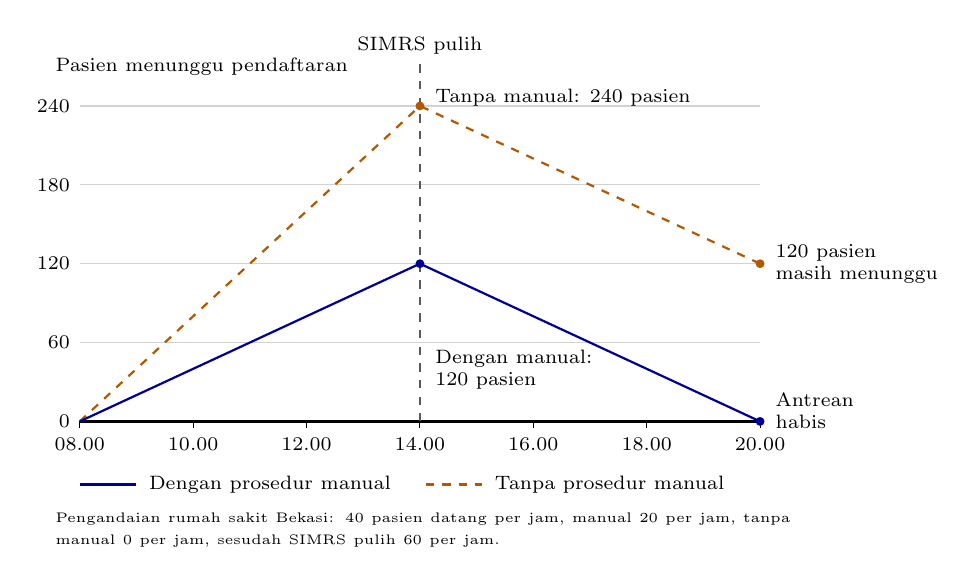
\begin{tikzpicture}[font=\scriptsize, x=0.72cm, y=0.0167cm]
  % Garis bantu dan sumbu: satu satuan x adalah satu jam, satu satuan y adalah satu pasien
  \foreach \nilai in {60,120,180,240} {
    \draw[gray!35] (0,\nilai) -- (12,\nilai);
    \node[left] at (0,\nilai) {\nilai};
  }
  \draw[thick] (0,0) -- (12,0);
  \node[left] at (0,0) {0};
  \foreach \posisi/\jam in {0/08.00,2/10.00,4/12.00,6/14.00,8/16.00,10/18.00,12/20.00} {
    \draw (\posisi,0) -- (\posisi,-5);
    \node[below] at (\posisi,-5) {\jam};
  }
  \node[anchor=south west] at (-0.6,256) {Pasien menunggu pendaftaran};
  % Penanda saat SIMRS kembali
  \draw[dashed, gray!70!black, thick] (6,0) -- (6,272);
  \node[above] at (6,272) {SIMRS pulih};
  % Seri tanpa prosedur manual
  \draw[orange!70!black, thick, dashed] (0,0) -- (6,240) -- (12,120);
  \fill[orange!70!black] (6,240) circle (1.6pt) (12,120) circle (1.6pt);
  \node[anchor=west] at (6.1,246) {Tanpa manual: 240 pasien};
  \node[anchor=west, align=left] at (12.1,120) {120 pasien\\masih menunggu};
  % Seri dengan prosedur manual
  \draw[blue!60!black, thick] (0,0) -- (6,120) -- (12,0);
  \fill[blue!60!black] (6,120) circle (1.6pt) (12,0) circle (1.6pt);
  \node[align=left, anchor=north west] at (6.1,62) {Dengan manual:\\120 pasien};
  \node[anchor=west, align=left] at (12.1,8) {Antrean\\habis};
  % Legenda
  \draw[blue!60!black, thick] (0,-48) -- (1,-48);
  \node[anchor=west] at (1.05,-48) {Dengan prosedur manual};
  \draw[orange!70!black, thick, dashed] (6.1,-48) -- (7.1,-48);
  \node[anchor=west] at (7.15,-48) {Tanpa prosedur manual};
  \node[anchor=north west, align=left, text width=9.6cm] at (-0.6,-62)
    {{\tiny\mdseries Pengandaian rumah sakit Bekasi: 40 pasien datang per jam, manual 20 per jam,
    tanpa manual 0 per jam, sesudah SIMRS pulih 60 per jam.}};
\end{tikzpicture}
